\subsection{Das konzeptionelles Modell der Webseite}
    Das konzeptionelle Modell wird in diesem Beispiel anahnd
    der Übersichtsseite des Studienportals \gls{babw} beschrieben.
    Abbildung \ref{image:findingTeachersModelOverview} zeigt einen
    Ausschnitt dieser Seite, auf dem die wichtigsten Bereiche zu sehen sind.
    Eine Darstellung des Modells ist in Abbildung
    \ref{image:findingTeachersModelUml} zu sehen.

    \begin{figure}[htb]
        \centering
        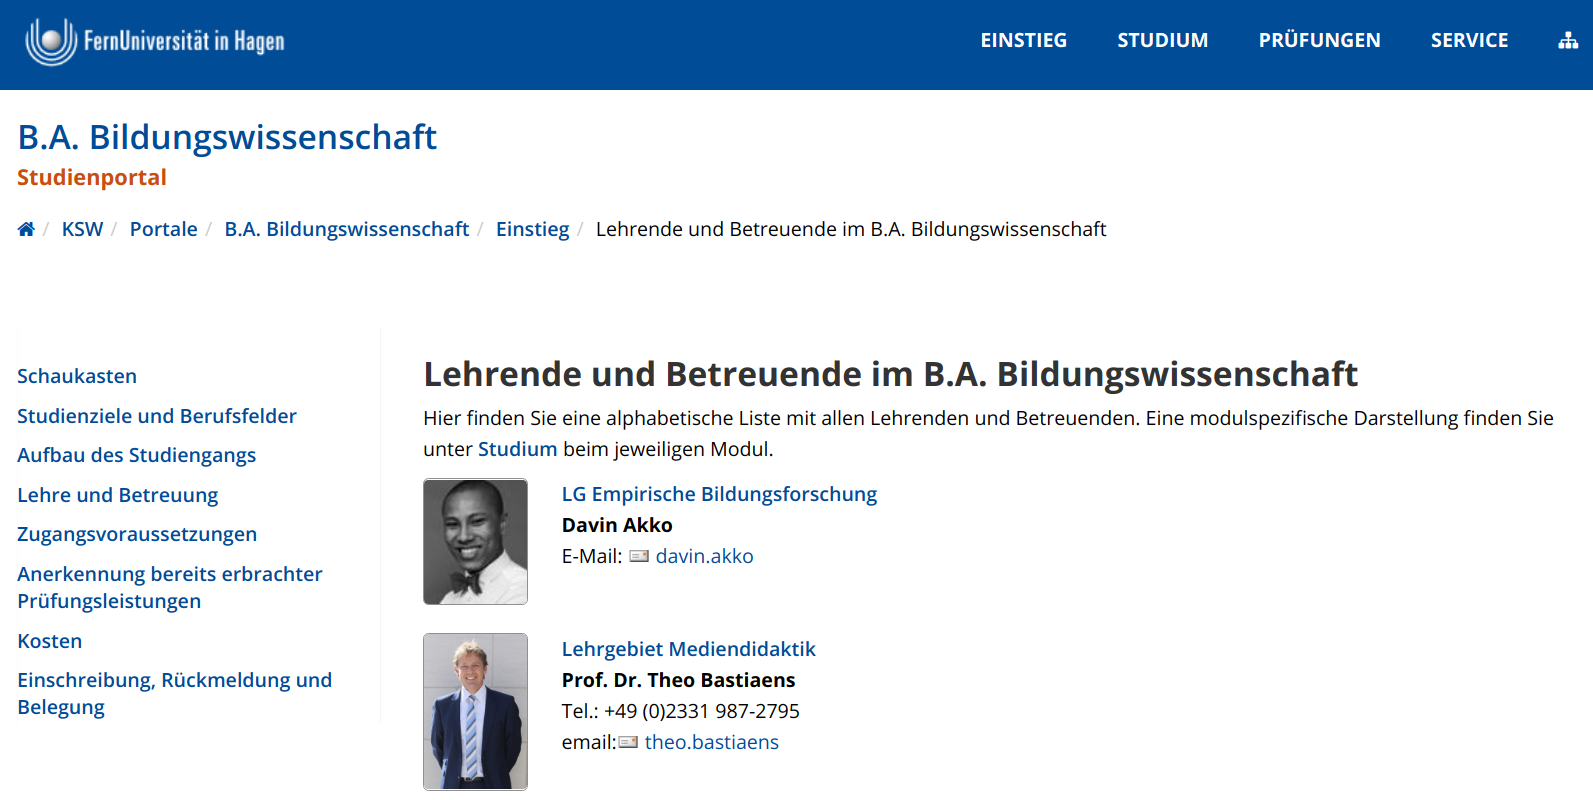
\includegraphics[width=\textwidth]{../resources/findings/case-study-1/model/overview.png}
        \caption{Lehrende und Betreuende im \gls{babw}}
        \label{image:findingTeachersModelOverview}
    \end{figure}

    Die Webseite lässt sich in verschiedene Bereiche aufteilen.
    Zunächst einen Kopfbereich, der auf der linken Seite das Logo
    der {\fernUni} enthält.
    Dieses Bild ist gleichzeitig ein Link zur Hauptseite der Universität. 
    Auf der rechten Seite enthält der Kopfbereich einige Links zu den verschiedenen
    Bereichen der Site.
    Direkt unter dem Kopfbereich befindet sich der Name des Studienportals,
    welcher gleichzeitig ein Link auf die Hauptseite der Website ist.
    Darunter befindet sich auf der linken Seite ein weiterer Navigationsbereich,
    der Verweise auf die Unterseiten des aktuellen Bereichs der Site enthält.
    Rechts daneben findet sich zunächst der Titel der Seite,
    gefolgt von einem kurzen einleitenden Absatz.
    Alle bisher genannten Elemente der Seite finden sich in sehr ähnlicher Form
    auch auf anderen Seiten der Site wieder.
    Die dem Absatz folgende Liste aller Lehrenden und Betreuenden unterscheidet die Seite hingegen von anderen.
    Für jeden Mitarbeiter sind eine Reihe an Informationen dargestellt.
    Neben einem Bild ist das der Name des Lehrgebiets, in dem er tätig ist.
    Dieser Name ist außerdem ein Link auf eine Seite über dieses Gebiet.
    Es folgen der Name des Mitarbeiters
    und einige Kontaktinformationen.
    Dies können eine E-Mail-Adresse, eine Telefonnummer
    und bei einigen wenigen Kontakten auch eine Faxnummer und ein Raum sein.

    \begin{figure}[htb]
        \centering
        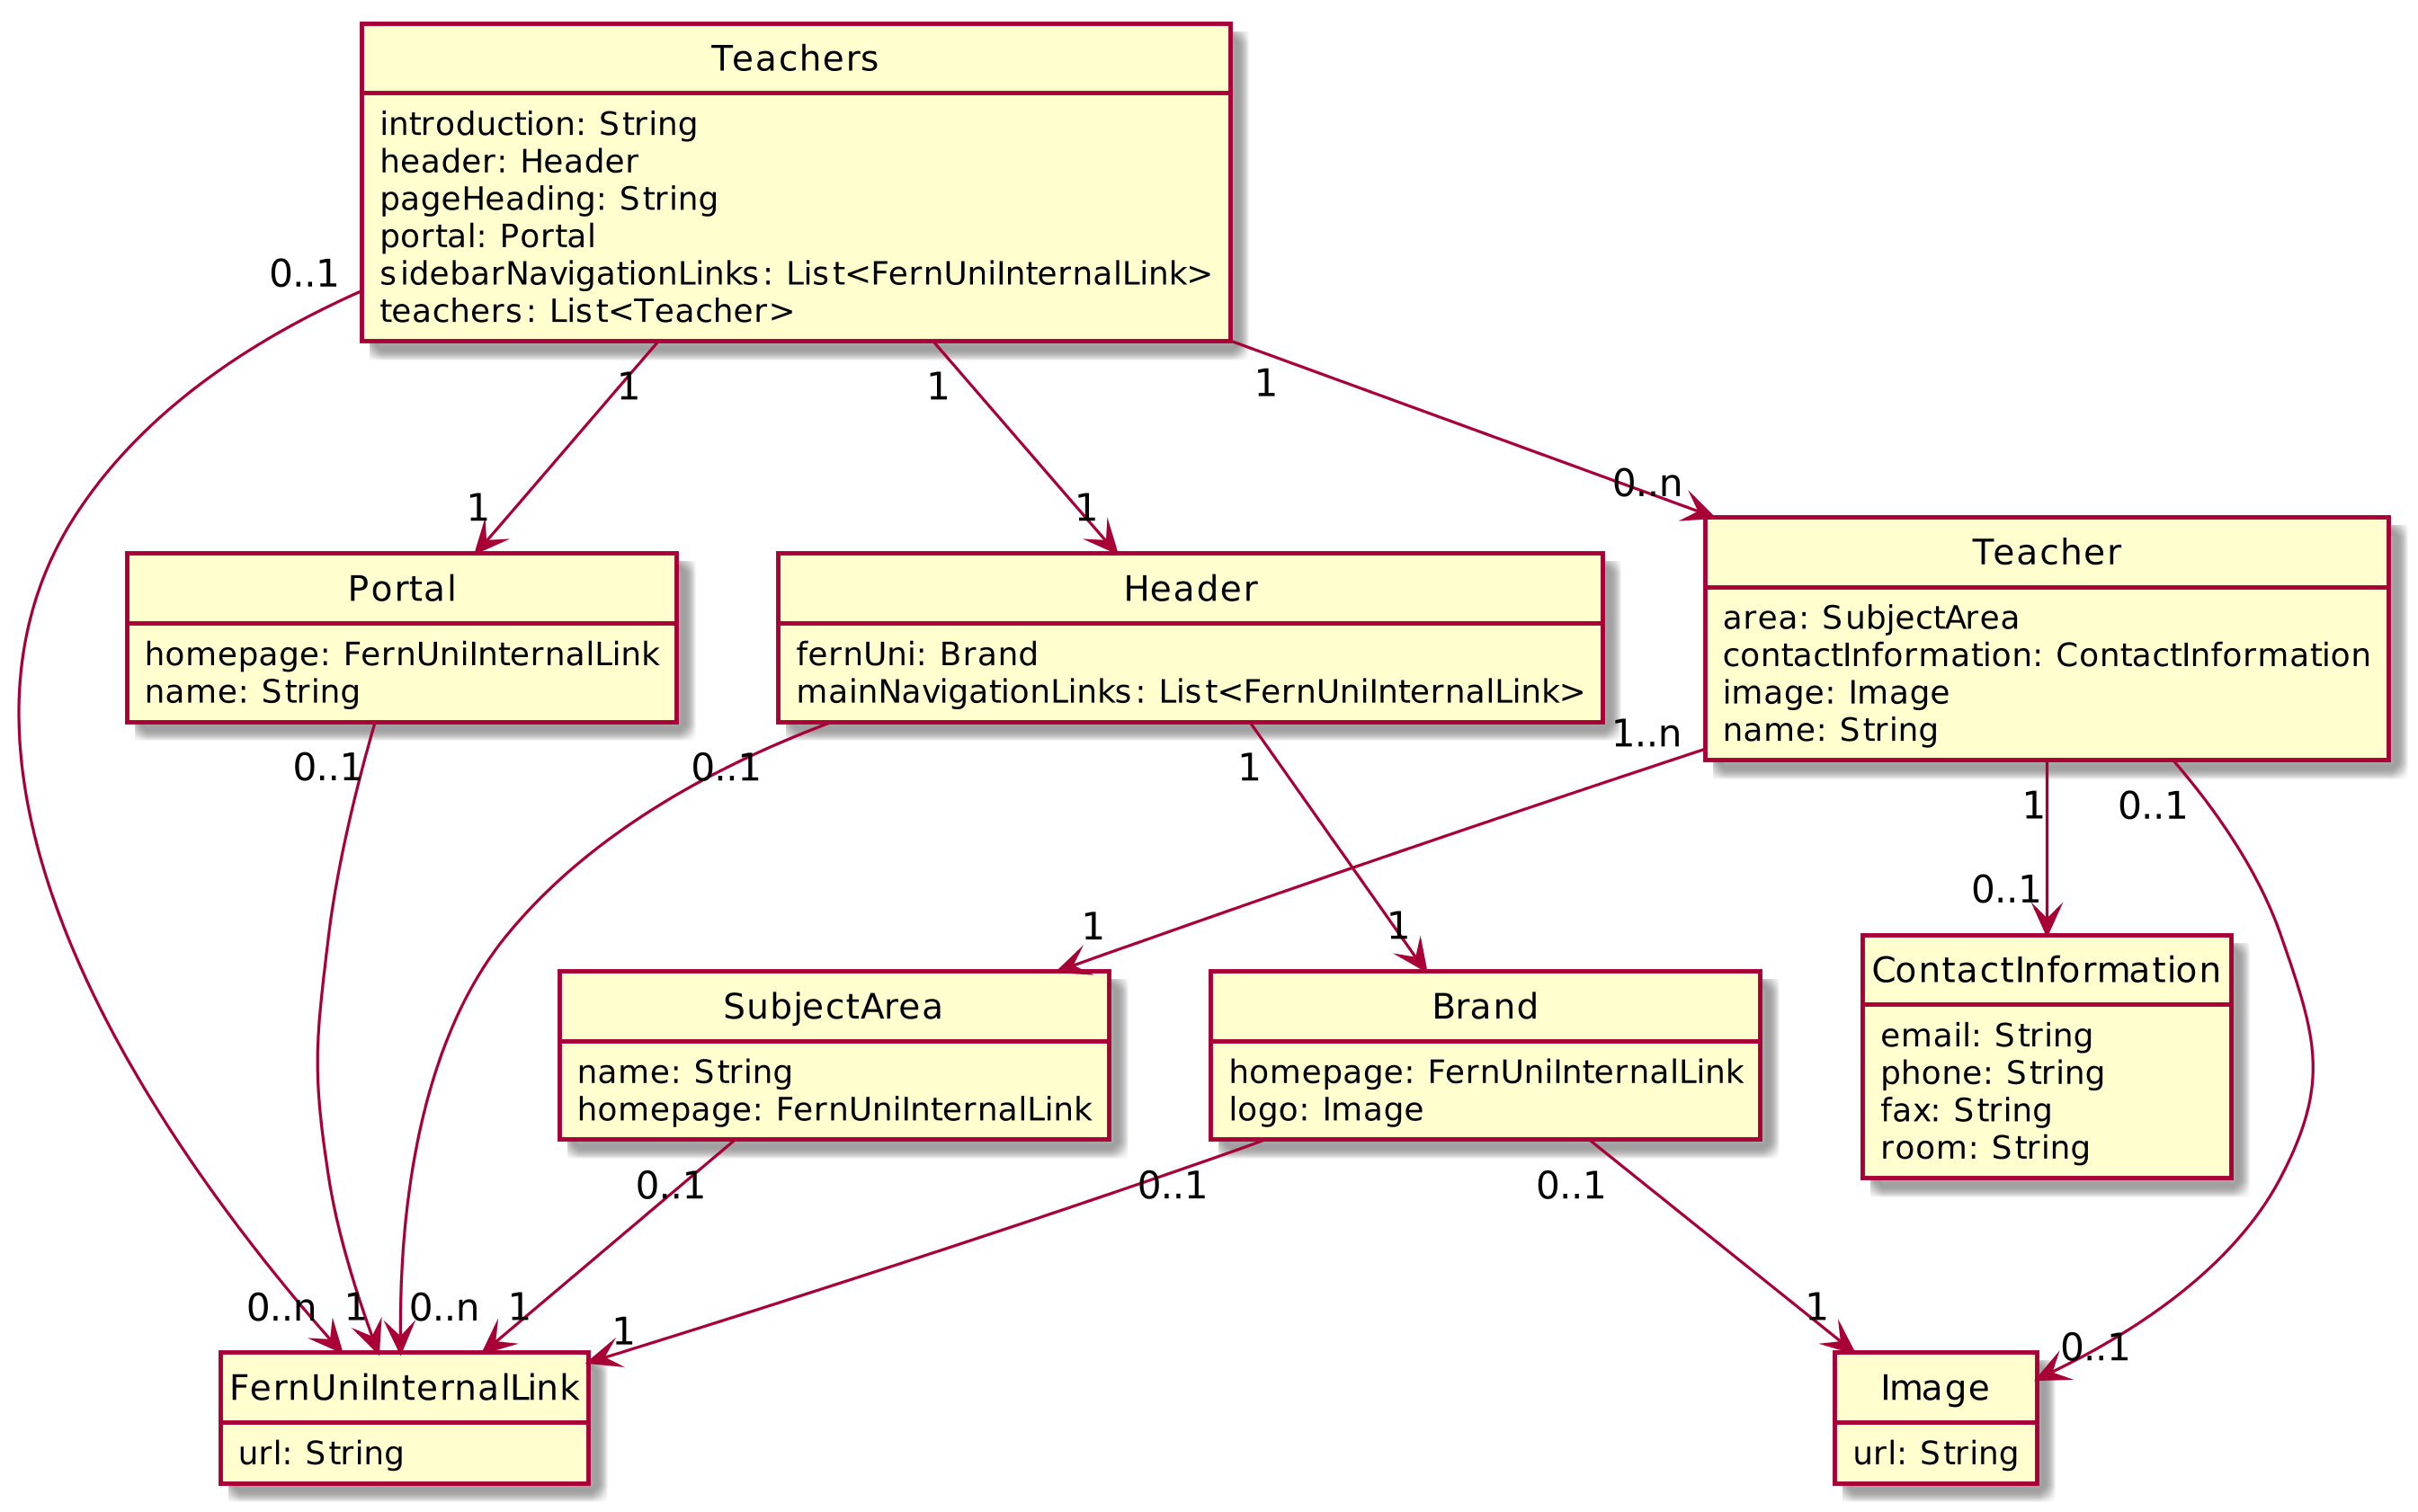
\includegraphics[scale=\imageScalingFactor]{../resources/findings/case-study-1/model/model.png}
        \caption{Konzeptionelles Modell der Seite über Lehrende und Betreuende}
        \label{image:findingTeachersModelUml}
    \end{figure}